\documentclass[size=11pt]{report}

\usepackage{authblk}
\usepackage{fancyhdr}
\usepackage{graphicx}
\usepackage{indentfirst}
\usepackage[portuguese]{babel}

\title{TP2}
\title{
    Comunicação por Computador \\
    \large{Trabalho Prático 3}
}

\author{
    Cristiano Pereira A93726 \\
    Marco Costa A93283 \\
    Hugo Fernandes A89481
}

\affil{
    Universidade do Minho \\
    Departamento de Informática
}


\begin{document}
    \maketitle
    \newpage

    \section*{Parte I}
        \subsection*{1}
            \noindent
            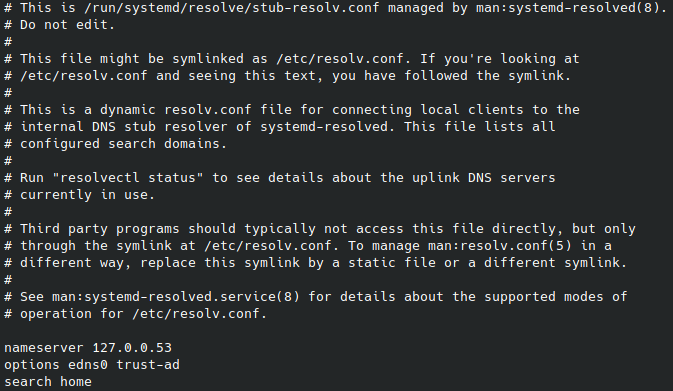
\includegraphics[width=\textwidth]{images/resolv.conf.png}
            \par
                O ficheiro \textit{/etc/resolv.conf} é lido pelas rotinas do resolver para saber
            a que servidor de DNS se deve conectar, bem como outras informações de configuração.\par 
                Na imagem acima pode ser visto todo o conteúdo deste ficheiro. Para além de várias linhas de comentários
            podem ser lidas três linhas que dizem ao \textit{resolver} como se comportar. Esta máquina foi configurada com os seguintes parâmetros: 
            \begin{description}
                \item[nameserver 127.0.0.53] Diz ao \textit{resolver} a que servidor DNS se deve conectar. Neste caso aponta para o endereço 127.0.0.53 no
                \textit{localhost} onde opera o processo \textit{systemd-resolved} que toma conta do processo de encaminhamento dos pedidos.
                \item[options edns0 trust-ad] Permite mudar as variáveis internas do \textit{resolver}.
                \item[search home]   
            \end{description}
            \pagebreak
        \subsection*{2}
                Através do programa \textit{dig} podemos fazer queries de DNS para saber se algum dos servidores \textbf{www.di.uminho.pt.} ou \textbf{www.europa.eu}
            tem algum endereço IPv6.\par
                Usamos o comando \textit{dig www.di.uminho.pt. AAAA} para procurar especificamente por endereços IPv6 e obtivemos a seguinte resposta:    
            \par
            \noindent
            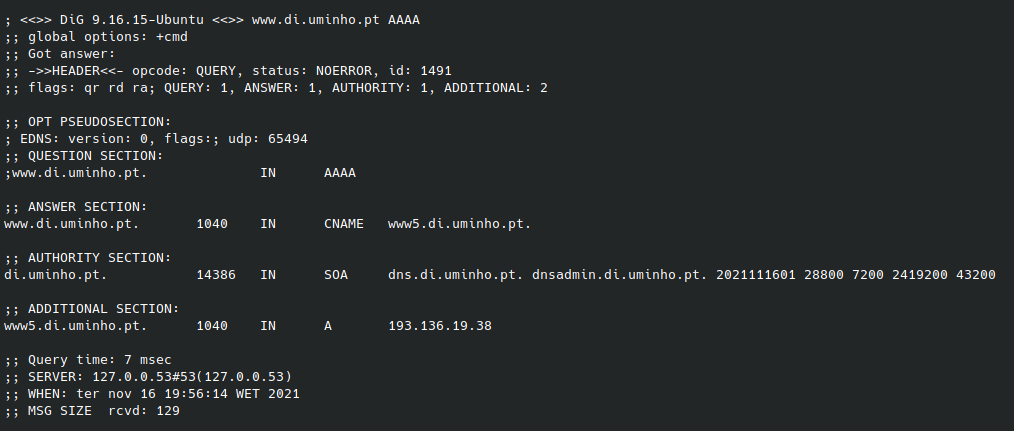
\includegraphics[width=\textwidth]{images/dig_di.png}
            \par
                A resposta que nos foi fornecida não inclui nenhuma entrada \textbf{AAAA} logo conluímos que este servidor não tem nenhum endereço IPv6.

                \vspace{0.45em}
                Por outro lado o output de \textit{dig www.europa.eu. AAAA} foi o seguinte:
            \par
            \noindent
            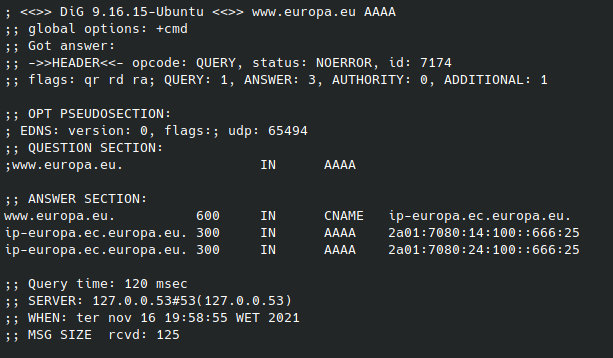
\includegraphics[width=\textwidth]{images/dig_europa.png}
            \par
                Esta resposta ao contrário da anterior mostra um \textbf{CNAME} que aponta para \textbf{ip-europa.ec.europa.eu.} e dois endereços IPv6 pertencentes a esse servidor.
\end{document}